% chapters/02_sections/cuda_programming_model.tex
\section{CUDA Programming Model}\label{sec:cuda}
CUDA (Compute Unified Device Architecture) is NVIDIA's parallel programming platform for general-purpose computation on GPUs. A CUDA program consists of host code, which runs on the CPU, and \emph{kernels}, which are functions launched from the host but executed in parallel across many GPU threads. The programmer specifies the parallelism by choosing a grid of thread blocks at launch time; the hardware then schedules those blocks onto the available SMs.

\subsection{Thread Hierarchy and Kernel Launch}\label{sec:cuda-threads}

CUDA organises parallel execution into a three-level hierarchy: \emph{grids}, \emph{thread blocks} (or simply \emph{blocks}), and \emph{threads}. A kernel launch creates a single grid, which is partitioned into blocks. Each block contains a fixed number of threads that execute concurrently on the same SM and can cooperate through shared memory and synchronisation barriers. Threads in different blocks cannot synchronise with each other during kernel execution.

Both the grid and each block can be specified with up to three dimensions, which provides a natural mapping for problems defined over multidimensional arrays. The dimensions are set via the \texttt{dim3} type, and each thread identifies its position using the built-in variables \texttt{threadIdx}, \texttt{blockIdx}, \texttt{blockDim}, and \texttt{gridDim}.

\begin{figure}[H]
  \centering
  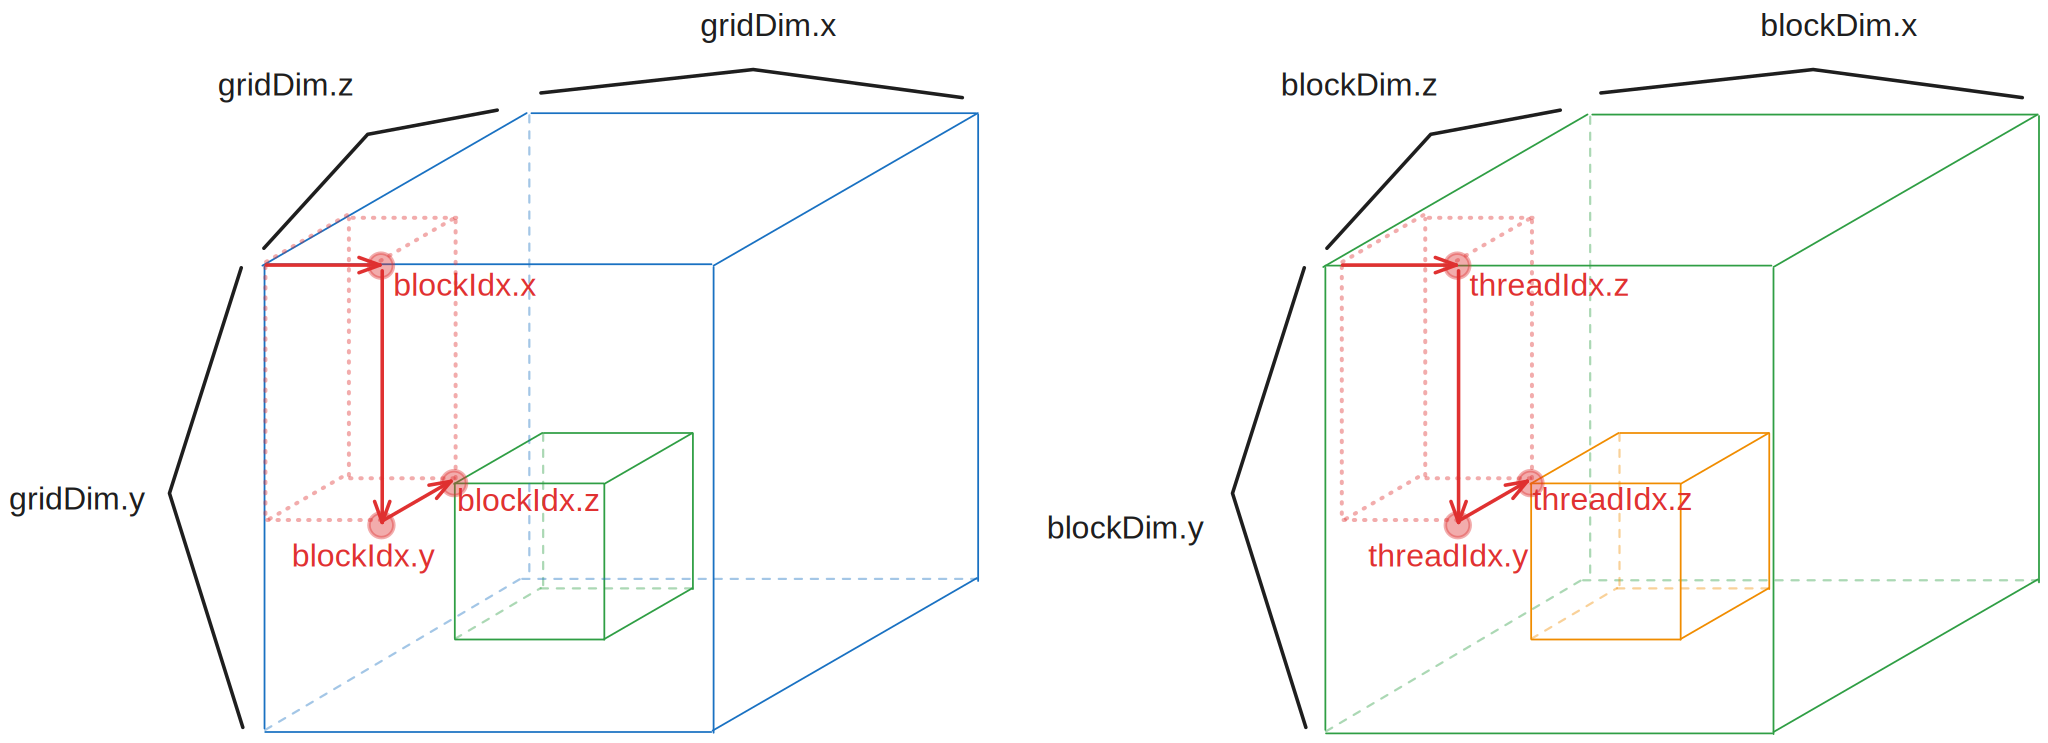
\includegraphics[width=0.85\textwidth]{GridBlockThreadAddressing}
  \caption{CUDA execution hierarchy showing the mapping of grids to thread blocks and threads. Threads are organised in up to three dimensions and identified using the built-in variables \texttt{threadIdx} and \texttt{blockIdx}.}
  \label{fig:cuda-thread-hierarchy}
\end{figure}

The hierarchical organisation of grids, thread blocks, and threads is illustrated in \cref{fig:cuda-thread-hierarchy}. Within each block, threads are further grouped into \emph{warps} of 32 threads that execute instructions in lock-step on the SM's SIMT (Single Instruction, Multiple Thread) execution units.

\subsubsection{Kernel Syntax and Launch Configuration}

A kernel is declared with the \lstinline[language=CUDA]{__global__} qualifier and launched using the triple-chevron syntax \texttt{<<<gridDim, blockDim>>>}. The following example illustrates a minimal kernel that adds two vectors element-wise:

\begin{lstlisting}[language=CUDA, caption={Element-wise vector addition kernel and its host-side launch.}, label={lst:vecadd}]
__global__ void vecAdd(const float *a, const float *b, float *c, int n) {
    int i = blockIdx.x * blockDim.x + threadIdx.x;
    if (i < n) {
        c[i] = a[i] + b[i];
    }
}

// Host launch
int n = 1 << 20;                    // 1,048,576 elements
int threadsPerBlock = 256;
int blocksPerGrid = (n + threadsPerBlock - 1) / threadsPerBlock;
vecAdd<<<blocksPerGrid, threadsPerBlock>>>(d_a, d_b, d_c, n);
\end{lstlisting}

The global thread index is computed on line~2 as \lstinline[language=CUDA]{blockIdx.x * blockDim.x + threadIdx.x}. This is the standard one-dimensional addressing pattern: \texttt{blockIdx.x} selects which block the thread belongs to, \texttt{blockDim.x} gives the number of threads per block, and \texttt{threadIdx.x} is the thread's position within its block. The bounds check on line~3 is necessary because the total number of threads launched (blocks $\times$ threads per block) is rounded up to a multiple of the block size and may therefore exceed~\texttt{n}.

\subsubsection{Two-Dimensional Grid Addressing}

For problems with a natural two-dimensional structure, such as matrix operations or image processing, both the grid and block dimensions can be specified in two (or three) dimensions. The following example demonstrates a kernel that transposes an $M \times N$ matrix:

\begin{lstlisting}[language=CUDA, caption={Matrix transpose using two-dimensional grid and block addressing.}, label={lst:transpose-2d}]
__global__ void transpose(const float *in, float *out, int M, int N) {
    int col = blockIdx.x * blockDim.x + threadIdx.x;
    int row = blockIdx.y * blockDim.y + threadIdx.y;
    if (row < M && col < N) {
        out[col * M + row] = in[row * N + col];
    }
}

// Host launch
dim3 blockDim(16, 16);          // 256 threads per block
dim3 gridDim(
    (N + blockDim.x - 1) / blockDim.x,
    (M + blockDim.y - 1) / blockDim.y
);
transpose<<<gridDim, blockDim>>>(d_in, d_out, M, N);
\end{lstlisting}

Here each thread is addressed by a \texttt{(row, col)} pair derived from the two-dimensional block and thread indices. The grid is sized so that at least $M \times N$ threads are launched, again with bounds checking to handle dimensions that are not exact multiples of the block size.

\subsubsection{Block Size Selection and Hardware Constraints}\label{sec:block-size}

The choice of block size affects both correctness and performance. The CUDA programming model imposes an upper limit of 1024 threads per block. Beyond this hard limit, several performance-relevant factors guide the choice:

\begin{itemize}
  \item \textbf{Warp granularity.} Because threads are scheduled in warps of 32, the block size should be a multiple of 32 to avoid partially filled warps whose unused lanes still consume scheduling resources.
  \item \textbf{Occupancy.} Each SM has a finite number of registers, a fixed amount of shared memory, and a maximum number of resident threads (\num{2048} on the A100). If a kernel uses many registers per thread, fewer threads can reside on the SM simultaneously, which may leave the hardware underutilised. The CUDA occupancy calculator relates block size and per-thread resource usage to the fraction of the SM's capacity that is occupied.
  \item \textbf{Shared memory per block.} Shared memory is partitioned among the blocks resident on an SM. A block that allocates a large amount of shared memory limits the number of blocks that can coexist, potentially reducing occupancy.
\end{itemize}

In practice, block sizes of 128 or 256 threads are common defaults that balance these constraints. More performance-critical kernels tune the block size empirically or use the \lstinline[language=CUDA]{__launch_bounds__} qualifier to give the compiler additional information for register allocation.

\subsubsection{Linearisation of Multidimensional Indices}\label{sec:linearisation}

GPU memory is addressed linearly, so multidimensional arrays must be mapped to one-dimensional offsets. For a tensor stored in row-major order, the linear index of element $(i, j)$ in an $M \times N$ matrix is
\begin{equation}\label{eq:row-major}
  \text{offset} = i \cdot N + j,
\end{equation}
which generalises to higher-order tensors by successive multiplication with trailing dimensions. In column-major (Fortran) order, the convention used by cuBLAS and most BLAS libraries, the index is instead
\begin{equation}\label{eq:col-major}
  \text{offset} = j \cdot M + i.
\end{equation}
\Cref{lst:transpose-2d} uses row-major layout for the input (\texttt{in[row * N + col]}) and column-major layout for the output (\texttt{out[col * M + row]}), which is precisely the transpose operation.

A concrete example: for a $4 \times 3$ matrix stored in row-major order, the element at row~2, column~1 maps to linear offset $2 \cdot 3 + 1 = 7$. Understanding this mapping is essential for implementing coalesced memory access patterns, discussed in \cref{sec:coalescing}.

\subsection{Shared Memory and Synchronisation}\label{sec:shared-memory}

Shared memory is an on-chip, programmer-managed memory space visible to all threads within a block. It serves two purposes: as a software-managed cache to stage data from global memory, and as a communication channel between threads in the same block. Because shared memory has much lower latency than global memory (approximately \num{20} cycles versus \num{500} cycles on the A100, cf.\ \cref{tab:a100-memory-latency}), its effective use is often the difference between a bandwidth-bound kernel and one that approaches peak compute throughput.

\subsubsection{Static and Dynamic Allocation}

Shared memory can be allocated statically at compile time or dynamically at launch time. Static allocation uses the \lstinline[language=CUDA]{__shared__} qualifier with a fixed array size:

\begin{lstlisting}[language=CUDA, caption={Static shared memory allocation for a tile.}, label={lst:shmem-static}]
__shared__ float tile[TILE_SIZE][TILE_SIZE];
\end{lstlisting}

Dynamic allocation is specified as a third argument in the launch configuration and accessed through an \lstinline[language=CUDA]{extern __shared__} declaration:

\begin{lstlisting}[language=CUDA, caption={Dynamic shared memory allocation.}, label={lst:shmem-dynamic}]
extern __shared__ float smem[];

// Host launch with dynamic shared memory size in bytes
kernel<<<grid, block, sharedBytes>>>(args);
\end{lstlisting}

Dynamic allocation is useful when the tile size depends on runtime parameters, which is common in autotuned kernels.

\subsubsection{Tiled Matrix Multiplication}\label{sec:tiled-matmul}

The canonical use of shared memory is tiled (or blocked) matrix multiplication. A na\"ive matrix multiplication kernel that computes $C = AB$ with $A \in \R^{M \times K}$ and $B \in \R^{K \times N}$ has each thread compute one element of $C$ by reading an entire row of $A$ and column of $B$ from global memory. This results in $\BigO(K)$ global loads per thread and an arithmetic intensity of roughly $2\;\text{FLOPs}/\text{byte}$---well below the A100's crossover point of $\approx 9.6\;\text{FLOPs}/\text{byte}$ for FP32 (\cref{tab:a100-derived}).

Tiling reduces global memory traffic by loading the input matrices into shared memory in small blocks (tiles), computing partial dot products from the tile, and then advancing to the next tile. \Cref{lst:tiled-matmul} shows the structure of this approach.

\begin{lstlisting}[language=CUDA, caption={Tiled matrix multiplication using shared memory. Each block computes one tile of the output matrix $C$.}, label={lst:tiled-matmul}]
#define TILE 16

__global__ void matmul(const float *A, const float *B, float *C,
                       int M, int N, int K) {
    __shared__ float As[TILE][TILE];
    __shared__ float Bs[TILE][TILE];

    int row = blockIdx.y * TILE + threadIdx.y;
    int col = blockIdx.x * TILE + threadIdx.x;
    float sum = 0.0f;

    for (int t = 0; t < (K + TILE - 1) / TILE; t++) {
        // Cooperative load: each thread loads one element of each tile
        int aCol = t * TILE + threadIdx.x;
        int bRow = t * TILE + threadIdx.y;
        As[threadIdx.y][threadIdx.x] = (row < M && aCol < K)
                                       ? A[row * K + aCol] : 0.0f;
        Bs[threadIdx.y][threadIdx.x] = (bRow < K && col < N)
                                       ? B[bRow * N + col] : 0.0f;

        __syncthreads();  // ensure the tile is fully loaded

        for (int k = 0; k < TILE; k++) {
            sum += As[threadIdx.y][k] * Bs[k][threadIdx.x];
        }

        __syncthreads();  // safe to overwrite tile in next iteration
    }

    if (row < M && col < N) {
        C[row * N + col] = sum;
    }
}
\end{lstlisting}

The kernel structure has three important properties:

\begin{enumerate}
  \item \textbf{Cooperative loading (lines 14--19).} Every thread in the block loads exactly one element of the $A$-tile and one element of the $B$-tile. The 256 threads in a $16 \times 16$ block therefore load the entire $16 \times 16$ tile cooperatively. Boundary conditions are handled by loading zero for out-of-range indices.
  \item \textbf{Barrier synchronisation (line 21).} The \lstinline[language=CUDA]{__syncthreads()} call ensures that all threads have finished writing to shared memory before any thread begins reading from the tile. A second barrier after the computation (line 27) prevents any thread from overwriting the tile before all threads have finished using it.
  \item \textbf{Data reuse.} Each element loaded into \texttt{As} is read by all 16 threads in its row; each element of \texttt{Bs} is read by all 16 threads in its column. This $16\times$ reuse from shared memory instead of global memory raises the effective arithmetic intensity by the tile size factor.
\end{enumerate}

For a tile size of $T$, the number of global memory loads per output element drops from $2K$ (na\"ive) to $2K/T$, and the arithmetic intensity increases proportionally by $T$. Larger tiles improve reuse but require more shared memory per block, which can limit occupancy.

\subsection{Memory Coalescing and Bank Conflicts}\label{sec:coalescing}

\subsubsection{Global Memory Coalescing}

When a warp executes a load or store instruction, the hardware combines the 32 individual thread addresses into as few memory transactions as possible. If consecutive threads access consecutive memory addresses (i.e.\ thread $i$ accesses address $\text{base} + i$), the accesses are \emph{coalesced} into a minimal number of 128-byte cache line transactions. Non-coalesced access patterns---strided or scattered---require multiple transactions for the same warp, wasting bandwidth.

Consider accessing a row-major $M \times N$ matrix. Iterating over columns (adjacent elements in memory) with consecutive threads produces coalesced accesses:

\begin{lstlisting}[language=CUDA, caption={Coalesced access pattern: consecutive threads read consecutive columns.}, label={lst:coalesced}]
// Coalesced: threads in a warp read adjacent elements
float val = matrix[row * N + threadIdx.x];
\end{lstlisting}

Iterating over rows with consecutive threads instead produces strided accesses with stride~$N$, which is poorly coalesced:

\begin{lstlisting}[language=CUDA, caption={Non-coalesced access pattern: consecutive threads read elements separated by stride $N$.}, label={lst:non-coalesced}]
// Non-coalesced: stride-N access
float val = matrix[threadIdx.x * N + col];
\end{lstlisting}

This distinction is particularly relevant for tensor contractions, where the choice of loop ordering and index layout determines whether the innermost memory accesses are contiguous or strided.

\subsubsection{Shared Memory Bank Conflicts}

Shared memory is divided into 32 \emph{banks}, each 4 bytes wide, interleaved in a round-robin fashion: word $k$ resides in bank $k \bmod 32$. When multiple threads in a warp access different words in the same bank simultaneously, the accesses are serialised into multiple rounds, creating a \emph{bank conflict}. The worst case is a 32-way bank conflict, where all threads hit the same bank, serialising the access entirely.

A common source of bank conflicts arises when accessing columns of a shared memory array whose leading dimension is a multiple of 32:

\begin{lstlisting}[language=CUDA, caption={Bank conflict when accessing a column of a 32-wide shared array, and the padding fix.}, label={lst:bank-conflict}]
// 32-way bank conflict: column access, stride = 32
__shared__ float tile[32][32];
float val = tile[threadIdx.x][col];  // threads 0..31 all hit same bank

// Fix: pad the leading dimension by one
__shared__ float tile[32][33];       // stride = 33, conflicts eliminated
float val = tile[threadIdx.x][col];
\end{lstlisting}

Adding one element of padding to the inner dimension changes the stride to 33, which is coprime to 32, so consecutive rows map to distinct banks. This is a standard optimisation in tiled kernels.

\subsection{Performance Profiling with Nsight Compute}\label{sec:nsight}

NVIDIA Nsight Compute is a kernel-level profiling tool for CUDA applications. It collects hardware performance counters and presents them as high-level metrics and roofline-model analyses, making it the primary tool for identifying performance bottlenecks in GPU kernels.

A typical profiling workflow proceeds as follows. First, the application is run under \texttt{ncu} (the Nsight Compute command-line interface), which replays each kernel multiple times to collect a full set of counters. Then the resulting report is examined either in the Nsight Compute GUI or by querying specific metrics from the command line.

Key metrics reported by Nsight Compute that are relevant to the optimisations discussed in subsequent chapters include:

\begin{itemize}
  \item \textbf{Achieved occupancy:} the ratio of active warps per cycle to the maximum the SM can support, indicating how effectively the kernel hides memory latency through parallelism.
  \item \textbf{Memory throughput:} the achieved bandwidth to each level of the memory hierarchy (HBM, L2, shared memory), compared against the theoretical peak. A kernel achieving close to peak HBM bandwidth is memory-bound.
  \item \textbf{Compute throughput:} the achieved FLOP/s relative to the peak, broken down by instruction type. A kernel well below peak compute with high memory throughput is bandwidth-limited.
  \item \textbf{Warp stall reasons:} a breakdown of why warps were stalled (e.g.\ waiting for memory, waiting at a barrier, instruction dependencies), which directly guides optimisation.
  \item \textbf{Shared memory bank conflicts:} the number of replayed shared memory accesses due to bank conflicts, indicating whether padding or access pattern changes are needed.
  \item \textbf{L2 cache hit rate:} the fraction of global memory requests served by the L2 cache, relevant for understanding data reuse across thread blocks.
\end{itemize}

Throughout the implementation chapters of this thesis, Nsight Compute profiles are used to validate performance models, confirm that kernels are operating in the expected regime (compute-bound or memory-bound), and guide iterative optimisation of tensor contraction kernels.

\subsection{Kernel Launch Mechanics}\label{sec:kernel-launch-mechanics}

The triple-chevron syntax \texttt{<<<gridDim, blockDim>>>} conceals a
multi-stage pipeline that spans both host and device~\cite{nvidia-cuda-guide}.
Understanding this pipeline is essential for reasoning about the cost of
launching many small kernels, which is the regime encountered in tensor network
contractions.

When the host executes a kernel launch, the following sequence of operations
takes place:

\begin{enumerate}
  \item \textbf{Argument marshalling.} The kernel's parameters---device
    pointers, scalars, dimensions---are packed into a parameter buffer and
    validated against the current CUDA context.
  \item \textbf{Command enqueueing.} The launch command, containing the kernel
    function pointer, grid and block dimensions, dynamic shared memory size,
    and the parameter buffer, is placed into the stream's command queue. The
    host-side API call returns immediately; the launch is \emph{asynchronous}
    from the host's perspective.
  \item \textbf{Driver serialisation.} The CUDA driver serialises the queued
    command into the GPU's hardware command buffer.
  \item \textbf{Block distribution.} The GPU's global block scheduler (referred
    to as the \emph{GigaThread engine} in NVIDIA's architecture
    whitepapers~\cite{nvidia2020a100}) dequeues the launch and begins
    distributing thread blocks to SMs. For each block, the scheduler verifies
    that the target SM has sufficient free resources---registers, shared
    memory, warp slots, and block slots---before making the assignment. Once
    assigned, a block remains on its SM until all of its warps complete
    execution; blocks do not migrate between
    SMs~\cite{nvidia-cuda-guide}.
  \item \textbf{Warp execution.} Within the assigned SM, the block's threads
    are partitioned into warps and handed to the processing block's warp
    scheduler, which begins issuing instructions as described in
    \cref{sec:sm-warps}.
\end{enumerate}

Steps 1--4 incur a fixed cost that is largely independent of the kernel's
computational workload. On the A100, this cost is typically in the range of
$5$--$10\;\mu\text{s}$ per launch. For large kernels that execute for
milliseconds, the overhead is negligible. For small kernels, however, the
launch cost can exceed the computation time by an order of magnitude or more.
This has a direct implication for workloads that require many small operations,
such as batches of low-dimensional GEMM calls arising from tensor
contractions: launching each operation as a separate kernel wastes the
majority of the wall-clock time on launch overhead rather than useful
computation.

\subsubsection{Kernel Fusion}\label{sec:kernel-fusion}

The standard mitigation for launch overhead is \emph{kernel fusion}: combining
multiple logically independent operations into a single kernel, so that the
launch cost is paid once rather than once per operation. In the context of this
thesis, fusion is achieved using cuBLASDx~\cite{cublasdx}, which provides a
device-side GEMM API that can be called from within a user-written kernel. This
allows multiple GEMM operations to be executed sequentially (or cooperatively)
inside a single kernel invocation, eliminating the per-operation launch cost
entirely. The cuBLASDx library is introduced in
\cref{sec:cublas-cublasdx-cutensor}, and the performance impact of fusion is
quantified experimentally in \cref{sec:launch-overhead-benchmark}.
